\documentclass{article}
\pdfpagewidth=8.5in
\pdfpageheight=11in

\usepackage{../WMHreport}
% Use the postscript times font!
\usepackage{times}
\usepackage{soul}
\usepackage{url}
\usepackage{xcolor}
\usepackage{polski}
\usepackage[polish]{babel}
\usepackage[utf8]{inputenc}
\usepackage[T1]{fontenc}
\usepackage[utf8]{luainputenc}
\usepackage[hidelinks]{hyperref}
\usepackage[utf8]{inputenc}
\usepackage{caption}
\usepackage{indentfirst}
\usepackage{graphicx}
\usepackage{amsmath}
\usepackage{siunitx}
\usepackage{booktabs}
\usepackage{listings,newtxtt}
\lstset{basicstyle=\ttfamily, keywordstyle=\bfseries}
\usepackage{subfig}

\urlstyle{same}
	
\title{Współczesne metody heurysytczne\\ Sprawozdanie cząstkowe}

\author{
Julia Kłos, Jakub Sikora
\affiliations
numery albumów: 283607, 283418 \\
\emails
julia.klos.stud@pw.edu.pl, jakub.sikora2.stud@pw.edu.pl
}

\newcommand{\todo}[1]{\textcolor{red}{\textbf{TO DO:} #1}}
\newcommand{\solve}[1]{\textcolor{blue}{\textbf{SOLVE:} #1}}
\begin{document}
\maketitle

\section{Opis problemu}
\label{sec:problem}
\\
Przedmiotem projektu jest znalezienie optymalnych parametrów maszyny wektorów nośnych (SVM-- \textit{Support Vector Machine}) w zagadnieniu aproksymacji. Aproksymowaną funkcją miała być dowolna ciągła funkcja dwuwymiarowa. W tym przypadku przyjęto funkcję określoną wzorem:
\begin{equation}
    \label{eqn:fun}
    f(x,y) = \log_{10}{|x|} \cos{y} + 0,55(x+y)
\end{equation}
\smallskip
\begin{figure}[h]
    \centering
    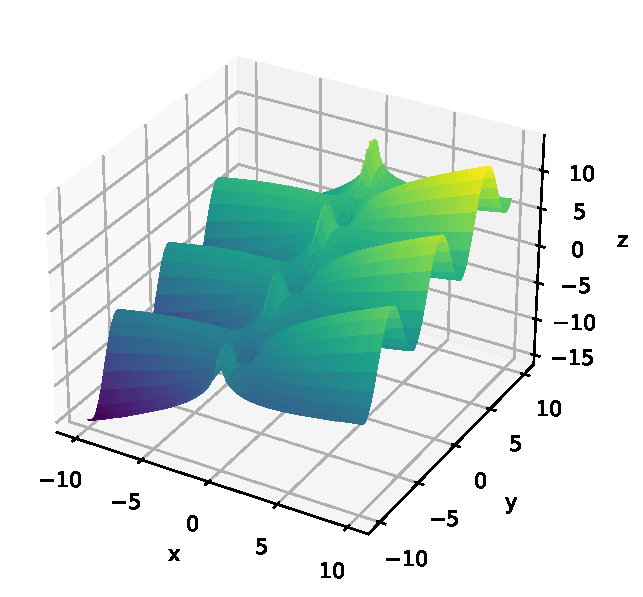
\includegraphics[width=0.5\textwidth]{assets/fun.pdf}
    \caption{Wykres aproksymowanej funkcji dwuwymiarowej}
    \label{fig:fun}
\end{figure}
W celu znalezienia optymalnych dla problemu parametrów zbadany zostanie wpływ poszczególnych parametrów algorytmu (funkcje jądrowe i ich atrybuty) na jakość klasyfikacji. Co więcej, aby sprawdzić, jak SVR (\textit{Support Vector Machine-- Regression}) poradziłby sobie dla rzeczywistych danych pomiarowych: zasymulowane zostaną one poprzez dodanie do aproksymowanej funkcji szumu. Zbadana zostanie jakość przybliżenia funkcji dla różnych poziomów szumu. 

Jako miary oceny działania algorytmu wybrano:
\begin{itemize}
    \item błąd średniokwadratowy ($MSE$)
    \item średni błąd względny ($MAE$),
    \item współczynnik determinacji ($R^2$).
\end{itemize}

        \begin{equation}
            \label{eqn:mse}
            MSE =\frac{1}{n} \sum_{i=1}^n (x_{i}-\hat{x}_{i})^2 \\[2ex]
        \end{equation}
        
        \begin{equation}
            \label{eqn:mae}
            MAE =\frac{1}{n} \sum_{i=1}^n \lvert x_{i}-\hat{x}_{i} \rvert \\[2ex]
        \end{equation}
        
        \begin{equation}
            \label{eqn:r2}
            R^{2} =1 - \frac{\sum_{i=1}^n (x_{i}-\hat{x}_{i})^2}{\sum_{i=1}^n (x_{i}-\bar{x}_{i})^2}   \\[2ex]
        \end{equation}
        
        \begin{array}{@{} l >{$}l<{$} @{}}
            n      & liczba pomiarów\\
            x_{i} & wartość rzeczywista\\
            \hat{x}_{i} & wartość przewidziana \\
            \bar{x}_{i} & wartość średnia $x$
        \end{array} \\[2ex]

\section{Opis algorytmów}
\label{sec:algorytm}
\\
\subsection{SVM}
\textit{Support Vector Machine}, czyli maszyna wektorów nośnych/podpierających, w podstawowej wersji stosowana jest do klasyfikacji poprzez znalezienie hiperprzestrzeni separującej z maksymalnym marginesem przykłady należące do różnych klas.
\begin{equation}
    y(x)= w^{T}x-b = 0
\end{equation}
Można zdefiniować równania decyzyjne:
\begin{equation}
    \begin{split}
    \label{eqn:decision}
     w^{T}x-b \geq 0,  d_{i}= +1\\
      w^{T}x-b < 0,  d_{i}= -1
     \end{split}
\end{equation}
\begin{array}{@{} l >{$}l<{$} @{}}
            w      & wektor wag\\
            x & wektor danych wejściowych\\
            b & polaryzacja \\
            d \in \{+1,-1\} & zdefiniowane klasy
 \end{array} \\[2ex]
 Co może zostać zapisane w postaci nierówności:
 \begin{equation}
   d_{i}(w^{T}x-b) >=1
 \end{equation}
  Spełniające je pary punktów $(x_{i}, d_{i})$ definiują wektory nośne (\textit{support vectors}), decydujące o położeniu hiperpłaszczyzny i szerokości marginesu separacji. Określenie decyzji wymaga wyznaczenia wektora wag oraz polaryzacji~\cite{zum}.
 
 Można wykazać, że  maksymalna odległość pomiędzy marginesami (\ref{eqn:decision}) wynosi $M= \frac{2}{\| w \|}$.Rozwiązanie dąży do maksymalizacji marginesu M, co oznacza minimalizowanie wektora $w$. Zagadnienie optymalizacji sprowadza się do minimalizowania po $w$ wyrażenia 
 \begin{equation}
 \label{eqn:minimum2}
     \frac{1}{2}\| w \|^2.
 \end{equation}

 
 Dla problemów nieseparowalnych liniowo występuje konieczność zmniejszenia marginesu separacji, co można zapisać przy użyciu nierówności:
 \begin{equation}
     d_{i}(w^{T}x-b)\geq 1 - \epsilon_{i} \
\end{equation}
 W tym przypadku określa się granicę decyzyjną dodatkowo poprzez minimalizowanie wartości $\epsilon_{i}$. Dla parametru  generalizującego $C$,deklarowanego przez użytkownika, dąży się do minimalizacji wyrażenia:
 \begin{equation}
 \frac{1}{2}\| w \|^2 + C\sum_{i=1}^n\epsilon_{i}
 \end{equation}

 \subsection{Funkcje jądrowe}
 Większość spotykanych problemów nie jest jednak liniowo separowalna. Aby móc skorzystać, pomimo tego, z algorytmu SVM, należy skorzystać z możliwości przetransformowania danych do przestrzeni o innym wymiarze, w której dane z dużym prawdopodobieństwem będą separowane liniowo. Dla przypadku nieliniowego funkcja decyzyjna opisana może zostać równaniem:
 \begin{equation}
 g(x) = w^{T}\phi(x)+b
 \end{equation}

 Najczęściej wykorzystywane funkcje jądrowe to:
 \begin{itemize}
      \item liniowa,
    \item wielomianowa,
    \item radialna (\textit{rbf}),
    \item sigmoidalna.
 \end{itemize}
 W tym zagadnieniu zazwyczaj wykorzystywana jest sztuczka jądrowa, która nie wymaga bezpośredniego transformowania atrybutów, a jedynie wyznaczania wartości funkcji jądrowej, bez definiowania nowych atrybutów.
 \subsection{SVR}
 \textit{Support Vector Regression} (SVR) wykorzystuje te same reguły co SVM, jednak do rozwiązywania problemów związanych z aproksymacją funkcji. 
 W regresji dąży się do minimalizowania błędu. Wykorzystując maszynę wektorów nośnych do tego zagadnienia, staramy się dopasować błąd do pewnego progu. Błąd jest minimalizowany (chociaż częściowo jest tolerowany), poprzez dopasowywanie hiperpłaszczyzny, maksymalizując margines.
 
W ramach projektu zbadany zostanie wpływ na wyniki regresji następujących parametrów:
\begin{itemize}
    \item wybranej funkcji jądrowej (liniowej, wielomianowej, radialnej i sigmoidalnej),
    \item parametr regularyzacji $C$,
    \item parametr marginesu błędu $\varepsilon$,
    \item parametr $\gamma$ (dla funkcji jądrowej: wielomianowej, radialnej i sigmoidalnej),
    \item stopień wielomianu $d$ (tylko wielomianowa),
    \item wyraz wolny $c_{0}$ (wielomianowa i~sigmoidalna).
\end{itemize}
\subsection{Algorytm ewolucyjny}
Algorytm ewolucyjny to metoda optymalizacyjna przeszukująca przestrzeń rozwiązań, którego idea została zaczerpnięta z ewolucji. Niezależnie od rozwiązywanego problemu, pojęcia związane z tą metodą zostały użyczone bezpośrednio z biologii. Kolejne generacje gatunku mają być jak najlepiej przystosowane do otaczającego środowiska, eliminując zaadaptowane osobniki. 

\textit{Osobniki}, czyli podstawowe jednostki (przykładowe rozwiązania) podlegające ewolucji, której celem jest stworzenie reprezentanta (znalezienie rozwiązania) możliwie najlepszego. \textit{Fenotypem} nazywamy wygląd zewnętrzy osobnika (czyli funkcja końcowa), a \textit{genotypem} zbiór informacji, stanowiący jego pełen opis. \textit{Populacja} to z kolei zespół osobników przebywających we wspólnym
środowisku. Genotyp jest stały w trakcie życia osobnika, a modyfikacje następują w wyniku rozmnażania. Fenotyp odzwierciedla dopasowanie osobnika do środowiska i to na jego podstawie dokonywana jest selekcja. Na zmiany w fenotypie wpływają zmiany w genotypie, które są głównie efektem krzyżowania osobników, chociaż mogą też wynikać z mutacji-- losowych, niewielkich zmian genotypu.

Algorytm rozpoczyna wybranie losowo pewnej populacji. Na podstawie ich dopasowania do środowiska, dokonywana jest selekcja-- najlepszym osobnikom umożliwia się reprodukcję. Genotypy wybranych osobników poddawane są krzyżowaniu, a dodatkowo losowo wprowadzane są mutacje. W ten sposób powstaje kolejne pokolenie, potencjalnie doskonalsze. Utrzymanie stałej liczby osobników w populacji umożliwia usuwanie najsłabszych osobników, ocenianych na podstawie fenotypu (funkcji go oceniającej). Jeśli nie zostanie spełnione kryterium stopu, powraca się do procesu reprodukcji.

Modyfikacje algorytmu ewolucyjnego uwzględniają różne definicje operacji krzyżowania, mutacji oraz selekcji. To co charakteryzuje tego typu algorytmy to szybkiego, równoległego przeszukiwania przestrzeni oraz uniknięcie pułapek minimum lokalnego.

\subsection{Reguły asocjacyjne}

Do interpretacji uzyskanych wyników, wykorzystany zostanie algorytm \emph{apriori} do indukcji reguł asocjacyjnych~\cite{agrawal1996fast}. Reguły asocjacyjne opisują cechy zbioru danych powiązanych ze sobą w~pewien sposób. Każda reguła ma postać:

\begin{center}
    Jeżeli \emph{poprzednik}, to \emph{następnik} 
\end{center}

Z~każdą regułą można związać dwie miary: wsparcia oraz ufności. Miara wsparcia opisuje jak często w~danym zbiorze danych, w~jednej transakcji, występują zarówno poprzednik oraz następnik reguły. Ufność reguły opisuje prawdopodobieństwo warunkowe pojawienia się następnika reguły, pod warunkiem że wystąpił jej poprzednik.

Podstawowym algorytmem automatycznej indukcji reguł asocjacyjnych jest algorytm \emph{apriori}. Opiera się on na generacji częstych zbiorów, których wsparcie jest większe niż założony próg. Algorytm generuje drzewo zbiorów, odcinając co iterację wszystkie zbiory uznane za nieczęste. Dzięki przycinaniu, algorytm znacząco zmniejsza liczbę przejść przez cały zbiór danych w~celu policzenia wsparcia.

Aby wygenerować reguły asocjacyjne ze zbioru danych numerycznych, należy te dane zdyskretyzować oraz zamienić do formatu transakcyjnego. Zdecydowaliśmy się na wprowadzenie wprowadzenie sztucznego podziału wartości $$U = \{maly, sredni, duzy\},$$
dzięki czemu otrzymane reguły będą czytelne i~proste do interpretacji~\cite{agrawal1996fast}.

\section{Plan eksperymentów}
W~ramach projektu wykonane zostaną trzy eksperymenty:
\begin{itemize}
    \item badanie ogólnego zachowania wskaźników jakości w~zależności od parametrów funkcji jądrowych,
    \item optymalizacja parametrów funkcji jądrowej w~celu uzyskania jak najlepszego modelu,
    \item badanie wpływu szumu na jakość modelu.
\end{itemize}

W~celu zbadania ogólnego zachowania wskaźników jakości w~zależności od parametrów funkcji jądrowych, wykorzystany zostanie algorytm przeszukiwania zupełnego po przestrzeni dostępnych parametrów. Badana przestrzeń zostanie podzielona w~taki sposób aby rozważać tylko punkty o~różnych rzędach wielkości. Dla każdego zestawu parametrów zostanie przygotowany model SVR, którego wskaźniki jakości zostaną obliczone za pomocą pięciokrotnej walidacji krzyżowej.

Do interpretacji uzyskanych wyników, zostaną wykorzystane reguły asocjacyjne. Takie podejście pozwoli na automatyczne wyciągnięcie wniosków na temat pożądanych wartości poszczególnych parametrów, w~przypadku gdy nie będzie możliwym wykreślenie charakterystyki na wykresie.

W~drugim kroku, za pomocą algorytmu ewolucyjnego dokonamy optymalizacji parametrów ze względu na badane wskaźniki jakości. Korzystając z~wiedzy z~pierwszego eksperymentu, zawęzimy przedział poszukiwanych parametrów, tak aby ograniczyć ilość potrzebnych obliczeń do minimum. Dla każdej badanej funkcji jądrowej, proces optymalizacji zostanie przeprowadzony ze względu na jeden z~badanych wskaźników jakości: błąd średniokwadratowy, średni błąd względny oraz współczynnik determinancji.

Tematem ostatniego eksperymentu, będzie zbadanie działania zoptymalizowanych modeli w~obliczu zaszumionych danych. Na oryginalną funkcję~\ref{fig:fun} zostanie nałożony biały, addytywny, gaussowski szum o~różnych poziomach mocy. Dla każdego badanego poziomu, zostaną zbadane wskaźniki jakości zarówno na zbiorze trenującym jak i~zbiorze walidacyjnym. Celem tego eksperymentu będzie określenie dla jakiego poziomu szumu model zaczyna znacząco tracić na swojej jakości.

\section{Założenia implementacyjne}
\label{sec:zalozenia}

Projekt zostanie zrealizowany głównie przy użyciu języka Python, wykorzystując środowisko Jupyter Notebook. Do generacji badanej funkcji oraz wszelkich obliczeń numerycznych zostanie użyty pakiet \textbf{numpy}~\cite{numpy}. Do tworzenia maszyn wektorów nośnych wykorzystany zostanie pakiet \textbf{scikit-learn}~\cite{scikit-learn}, który udostępnia moduł \textbf{svm}, w~którym znajdują się obiekty \textbf{SVM} (do klasyfikacji) oraz \textbf{SVR} (do regresji). 

\begin{lstlisting}[language=Python, captionpos=b, caption=Nagłówek klasy sklearn.svm.SVR]
class sklearn.svm.SVR(*, kernel='rbf', 
      degree=3, gamma='scale', 
      coef0=0.0, tol=0.001, C=1.0, 
      epsilon=0.1, shrinking=True, 
      cache_size=200, verbose=False, 
      max_iter=-1)
\end{lstlisting}

Pakiet ten udostępnia również moduł \textbf{model\_{}selection}, pozwalający na badanie jakości przygotowanych modeli, przeprowadzanie walidacji krzyżowej (funkcja \textbf{cros\_{}val\_{}score} oraz przeszukiwania zupełnego po dostarczonej przestrzeni parametrów (obiekt \textbf{GridSearchCV}. Zostanie on wykorzystany do przeprowadzenia pierwszego eksperymentu, czyli określenia zakresu poszukiwanych parametrów optymalnej maszyny wektorów nośnych. Generacja reguł asocjacyjnych zostanie wyjątkowo wykonana za pomocą języka R, wykorzystując do tego funkcję \textbf{apriori} z~pakietu~\textbf{arules}~\cite{arules}.

\begin{lstlisting}[language=Python, captionpos=b, caption=Nagłówek klasy model\_{}selection.GridSearchCV]
class model_selection.GridSearchCV(
      estimator, param_grid, *, 
      scoring=None, n_jobs=None, 
      refit=True, cv=None, verbose=0, 
      pre_dispatch='2*n_jobs',
      error_score=nan, 
      return_train_score=False)
\end{lstlisting}


Drugi eksperyment zostanie wykonany za pomocą algorytmu ewolucyjnego, zaimplementowanego w~bibliotece \textbf{scipy.optimize}~\cite{scipy}. Polecenie \textbf{differential\_{}evolution} pozwala na dokładne sterowanie procesem optymalizacji oraz podanie własnej funkcji celu, dzięki czemu możliwym jest badanie różnych wskaźników jakości. 

\begin{lstlisting}[language=Python, captionpos=b, caption=Nagłówek funkcji optimize.differential\_{}evolution]
def optimize.differential_evolution(
    func, bounds, args=(), tol=0.01, 
    strategy='best1bin', maxiter=1000, 
    popsize=15, mutation=0.5, 
    seed=None, callback=None, 
    disp=False, polish=True, 
    recombination=0.7, atol=0, 
    updating='immediate', 
    workers=1, constraints=())
\end{lstlisting}

Oprócz wymienionych wyżej pakietów i~bibliotek, do realizacji projektu wykorzystane zostaną biblioteki:
\begin{itemize}
    \item \textbf{pandas} -- wysokopoziomowa obsługa zbiorów danych, udostępnia obiekt \textbf{DataFrame},
    \item \textbf{matplotlib} -- generacja i~zapisywanie wykresów,
    \item \textbf{virtualenv} -- wirtualizacja środowiska i~zarządzanie pakietami.
\end{itemize}
\section{Stan pracy}
\subsubsection{Badanie wpływu parametrów funkcji jądrowych na wskaźniki jakości modelu}
Przeprowadziliśmy badania czterech funkcji jądrowych oraz wpływu ich parametrów na trzy różne wskaźniki jakości. W~tabeli~\ref{tab:modele} porównane zostały konkretne funkcje, badane parametry oraz liczbę policzonych modeli.

\begin{table}[tb]
 \centering
 \begin{tabular}{||c c c||} 
 \hline
 funkcja jądrowa & parametry & liczba modeli \\ [0.5ex]
 \hline\hline
 liniowa & $C$,$\varepsilon$ & 125  \\ 
 \hline
 rbf & $C$,$\varepsilon$,$\gamma$ & 625 \\
 \hline
 wielomianowa & $C$,$\varepsilon$, $d$, $c_{0}$ & 3125 \\
 \hline
 sigmoidalna & $C$,$\varepsilon$, $\gamma$, $c_{0}$ & 3125 \\
 \hline 
\end{tabular}

 \caption{Porównanie badanych funkcji jądrowych \label{tab:modele}}
\end{table}

Dla funkcji liniowej, która ma tylko dwa stopnie swobody, możliwym jest wykreślenie zależności danego wskaźnika jakości od parametrów $C$ oraz $\varepsilon$. Zależności te zostały wykreślone na rysunkach~\ref{fig:mse} oraz~\ref{fig:r2}.

\begin{figure}[h]
    \centering
    \includegraphics[width=0.5\textwidth]{assets/linear-mse.pdf}
    \caption{Wartość MSE w~zależności od $C$ oraz~$\varepsilon$}
    \label{fig:mse}
\end{figure}

\begin{figure}[h]
    \centering
    \includegraphics[width=0.5\textwidth]{assets/linear-r2.pdf}
    \caption{Wartość $R^2$ w~zależności od $C$~oraz~$\varepsilon$}
    \label{fig:r2}
\end{figure}

Dla wyników przeszukiwania odnoszących się do pozostałych funkcji jądrowych, wygenerowane zostały reguły asocjacyjne. Najciekawsze reguły zostały przedstawione w tabeli~\ref{tab:reguly}.

Kod realizujący przeszukiwanie zupełne po podanej przestrzeni parametrów został zamieszczony w~notatniku \texttt{Projekt-WMH.ipynb} natomiast analiza wyników została przeprowadzona w~notatniku \texttt{GridSearchResults.ipynb}. Indukcja reguł odbyła się przy użyciu języka~R, skrypt wykonujący to zadanie można znaleźć pod ścieżką \texttt{rules-induction/rules.R}.

\subsubsection{Optymalizacja modeli algorytmem ewolucyjnym}
Na podstawie wyników z~poprzedniej sekcji, ustaliliśmy sensowne przedziały dla każdego badanego parametru i~następnie uruchomiliśmy proces optymalizacji algorytmem ewolucyjnym. Na moment tworzenia tego dokumentu, udało nam się znaleźć optymalne parametry maszyny wektorów nośnych dla liniowej i~radialnej funkcji jądrowej. Wyniki działania procesu optymalizacji, wraz z~odpowiadającymi im wskaźnikami jakości, zostały przedstawione w~tabeli~\ref{tab:optim}. Podane wskaźniki jakości zostały obliczone \textbf{na zbiorze testowym}.

\begin{table}[h]
 \centering
 \begin{tabular}{||c c c c||} 
 \hline
 parametry & MAE & MSE & $R^2$ \\ [0.5ex]
 \hline\hline
 $C=64,76$, $\varepsilon=0,0067$ & $2,18\mathrm{e}{-3}$ & $7,173\mathrm{e}{-6}$ & $0,99$ \\ 
 \hline
 $C=21,62$, $\varepsilon=0,0134$ & $4,36\mathrm{e}{-3}$ & $2,856\mathrm{e}{-5}$ & $0,99$ \\ 
 \hline
 $C=6,092$, $\varepsilon=2,85\mathrm{e}{-3}$ & $9,13\mathrm{e}{-4}$ & $1,246\mathrm{e}{-6}$ & $0,99$ \\ 
 \hline

\end{tabular}

\caption{Wyniki procesu optymalizacji wskaźników jakości za pomocą algorytmu ewolucyjnego dla liniowej funkcji jądrowej \label{tab:optim}}
\end{table}

\begin{table*}[t]
 \centering
 \begin{tabular}{||c c c c||} 
 \hline
 poprzednik & następnik & wsparcie & ufność \\ [0.5ex]
 \hline\hline
 kernel=linear, C=small, epsilon=small & mean\_{}train\_{}mse=big & 0,133 & 0,666 \\ 
 \hline
 kernel=linear, C=small, epsilon=small & mean\_{}train\_{}mae=big & 0,133 & 0,666 \\ 
 \hline
 kernel=linear, C=small, epsilon=small & mean\_{}train\_{}r2=big & 0,133 & 0,666 \\ 
 \hline
 kernel=poly, C=big, coef0=small, degree=big, epsilon=small & mean\_{}test\_{}mae=small & 0,075 & 1,0 \\ 
 \hline
 kernel=poly, C=small, coef0=big, degree=small, epsilon=small & mean\_{}test\_{}mae=big & 0,05 & 1,0 \\ 
 \hline
 kernel=poly, C=big, coef0=big, degree=big, epsilon=small & mean\_{}fit\_{}time=big & 0,05 & 0,666 \\
 \hline
 kernel=rbf, C=big, epsilon=small, gamma=big & mean\_{}train\_{}mae=big & 0,144 & 1,0 \\
 \hline
 kernel=rbf, C=big, epsilon=small, gamma=big & mean\_{}test\_{}r2=big & 0,144 & 1,0 \\
 \hline
 kernel=rbf, C=big, epsilon=small, gamma=big & mean\_{}fit\_{}time=big & 0,144 & 1,0 \\
 \hline
 kernel=sigmoid, C=big, epsilon=small, coef0=small & mean\_{}train\_{}r2=big & 0,072 & 0,75 \\
 \hline
 kernel=sigmoid, C=small, epsilon=small, coef0=big & mean\_{}train\_{}mae=big & 0,064 & 0,666 \\
 \hline
 kernel=sigmoid, C=small, epsilon=small, gamma=small & mean\_{}fit\_{}time=big & 0,064 & 0,666 \\
 \hline
\end{tabular}

\caption{Najciekawsze odnalezione reguły asocjacyjne \label{tab:reguly}}
\end{table*}



\bibliographystyle{abbrv}
\bibliography{bibliography}
\end{document}